\documentclass[12pt]{article}
% or use the epsfig package if you prefer to use the old commands
\usepackage{epsfig}
\usepackage{hyperref}
\usepackage{listings}
\usepackage{graphicx}%
\usepackage{color}
\usepackage{hyperref}
\usepackage{setspace}


%%%% UNCOMMENT NEXT BLOCK FOR CRAMMING LOTS OF TEXT ONTO PAGE
 \topskip -1cm % cram
   \oddsidemargin 5mm
   \evensidemargin 5mm
   \topmargin   -1.4cm   %1 in. from top
   \textheight 24cm % 26cm % 23cm % 22cm  (cram a bit more on the page)
   \textwidth 15.5cm
%   \parindent 0.5cm


%\newcommand{\docdb}[1]{\href{http://dayabay.ihep.ac.cn/cgi-bin/DocDB/ShowDocument?docid=#1}{\color{blue}doc-{#1}}}
\newcommand{\COtwo}{${\rm CO}_2$}

\begin{document}


\title{Estimated cost of Belle II collaboration meetings and control room shifts}

\author{David E. Jaffe \\ BNL}
\date{\today}
\maketitle
\begin{abstract}
{
I present estimates of the cost of air fare and the quantity of \COtwo\ produced by air travel for Belle II General Meetings and Control Room shifts. 
}
\end{abstract}


%\doublespacing
\onehalfspacing   %%%% GLOBAL CHANGE OF SPACING

\section{Introduction}

I wanted to understand the costs and climate impact of Belle II-related travel. 

\section{Methodology}

I extracted collaborator names, institutions, institutional location and other information from spreadsheets of Belle II collaborator and institutions obtained from \href{https://b2mms.belle2.org/pls/apex/f?p=1546:18:12868551837158:::::}{\color{blue}B2MMS} on 20 September 2019. 

Attendance information for the $16^{\rm th}$ to the $34^{\rm th}$ B2GMs was obtained from html downloaded from the appropriate ``Participant list" from \href{indico.belle2.org}{\color{blue} indico.belle2.org} or \href{kds.kek.jp/indico}{\color{blue}kds.kek.jp/indico}. 

 Shifter information was obtained from html downloaded from the CR Captain and Navigator calendars at \href{https://shift.belle2.org}{\color{blue}shift.belle2.org}. 
 I did not attempt to assess the costs and climate impact of BCG and detector expert shifters.
 
 I obtained air fare information from \href{kayak.com}{\color{blue}kayak.com} for travel between home institutions and Tokyo on 29 September 2019 for travel dates 10-26 October 2019 or on 13 Oct 2019 for travel dates 10-26 November 2019. 
 I acknowledge that these fares may not be representative of costs for earlier or later B2GMs or shifts outside these time periods. 
 These fares are used to estimate the air fare for the round-trip travel of B2GM attendees or CR shifters. 
 
 I used the  \href{https://www.icao.int/environmental-protection/CarbonOffset/Pages/default.aspx}{\color{blue}ICAO Carbon Emission Calculator} to obtain the estimated \COtwo\ in kg for round-trip air travel between home institutions and Tokyo in October 2019. 
 The ICAO is the International Civil Aviation Organization of The United Nations. 
 The Calculator takes into account multi-leg travel between airports using known aircraft fuel consumption and passenger capacities. 

I plotted and fitted the \COtwo\ emission and round-trip travel distance for non- and one-stop air travel from Belle II home institutions to Tokyo as shown in Figure~\ref{fig:legs}. The fit assumes a linear dependence between round-trip air travel distance and \COtwo\ emission. 
I used these two parameterizations to estimate the \COtwo\ emission based on the travel distance from Belle II home institutions to Tokyo. 

I assumed all collaborators from Japanese institutions would not use air transportation and assigned no \COtwo\ emission or air fare costs.

Some B2GM attendees do not appear in \href{https://b2mms.belle2.org/pls/apex/f?p=1546:18:12868551837158:::::}{\color{blue}B2MMS}. 
For some B2GM attendees, it was not possible to easily and unambiguously match their name to the name of a Belle II collaborator in \href{https://b2mms.belle2.org/pls/apex/f?p=1546:18:12868551837158:::::}{\color{blue}B2MMS}. 
Lack of an institution name or use of alternative spelling or naming in the B2GM participants complicates matching. 

\begin{figure}[htbp]
\begin{center}
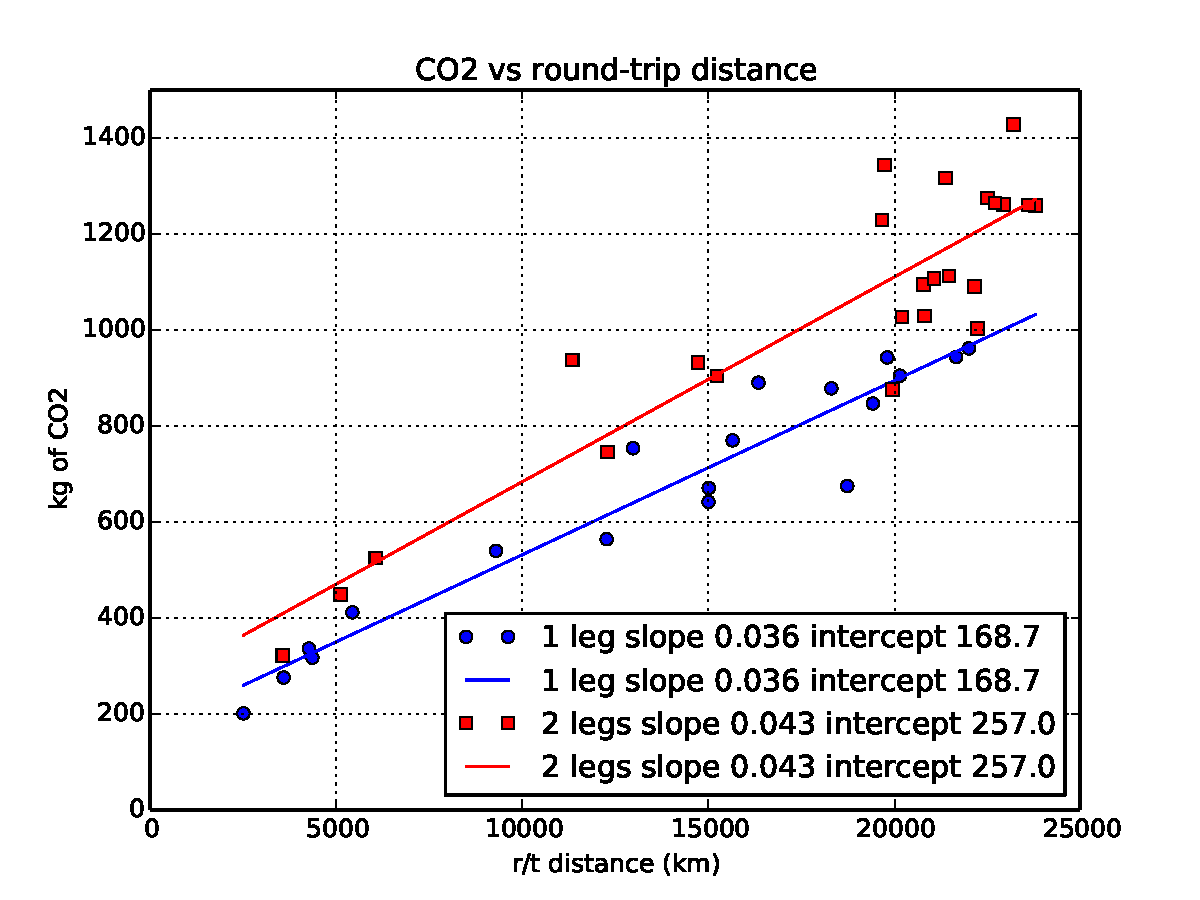
\includegraphics[width=\textwidth]{../FIGURES/all_legs.pdf}
\caption{\COtwo\ in kg {\sl vs.} air travel round-trip distance in km for single-leg (non-stop) and two-leg (one-stop) air travel from Belle II home institutions to Tokyo. The results of linear fits to the two groups are shown.}
\label{fig:legs}
\end{center}
\end{figure}

The statistics for B2GMs are shown in Table~\ref{tab:B2GM}. In the table, the `actual totals' are the sum for attendees that are not 'unknown' or 'bad'. 
The 'estimated totals' scale the `actual totals' by the ratio of the `bad' to 'actual' shifters. 
The total participants, fares, \COtwo\ and round-trip distances for the B2GMs are shown in 
Figures~\ref{fig:B2GM_part}, \ref{fig:B2GM_fares}, \ref{fig:B2GM_COtwo} and \ref{fig:B2GM_r-t}, respectively. 


The statistics for CR shifters are shown in Table~\ref{tab:Shifts}.
The totals for shifters, fares, \COtwo\ and distances are shown in 
Figures~\ref{fig:Shifts_part}, \ref{fig:Shifts_fares}, \ref{fig:Shifts_COtwo} and \ref{fig:Shifts_r-t}, respectively. 
For shifters, the estimated minima assume that each participating shifter only makes one round-trip journey per shift period. 
The estimated maxima assumes that each participating shifter makes a round-trip journey for each set of non-temporally-contiguous shifts. 
For example, if Jane Boggs had shifts M-Th for weeks 2, 3 and 4 of the shift period, Jane would be assumed to make three round-trip journeys for the estimated maximum and a single round-trip journey for the estimated minimum. 


\begin{table}[htp] 
\setlength{\tabcolsep}{2pt} 
\begin{center} 
\begin{tabular}{|rrrr| rrr| rrr| c|} 
\hline 
\multicolumn{4}{|c|}{Participants} & \multicolumn{3}{c|}{Actual totals} & \multicolumn{3}{c|}{Estimated totals} & \\ 
 att&japn& unk& bad&fares(USD)&   CO2(kg)&  r/t (km)& Fare(USD)&   CO2(kg)&  r/t (km)&Event \\ 
\hline 
 205&  43&   0&  30&    162852&    112849&   2287508&    199864&    138497&   2807396&16th B2GM \\ 
 181&  42&   1&  28&    133068&     92333&   1842300&    166940&    115836&   2311249&17th B2GM \\ 
 179&  41&   0&  26&    136619&     94938&   1906729&    168334&    116977&   2349362&18th B2GM \\ 
 228&  49&   0&  27&    181971&    127511&   2560749&    214295&    150161&   3015619&19th B2GM \\ 
 181&  40&   0&  19&    150091&    103349&   2070154&    173466&    119445&   2392554&20th B2GM \\ 
 202&  49&   0&  21&    165990&    112918&   2274690&    192398&    130883&   2636573&21st B2GM \\ 
 203&  46&   0&  17&    181558&    121921&   2459727&    203604&    136726&   2758408&22nd B2GM \\ 
 202&  49&   0&  13&    170468&    117044&   2335776&    186297&    127913&   2552670&23rd B2GM \\ 
 213&  51&   0&  12&    182096&    128721&   2604157&    196664&    139018&   2812489&24th B2GM \\ 
 219&  51&   0&  12&    186618&    130139&   2615049&    200973&    140150&   2816207&25th B2GM \\ 
 232&  58&   1&  11&    202133&    137541&   2758872&    215858&    146881&   2946202&26th B2GM \\ 
 239&  61&   0&   4&    204311&    142425&   2834062&    209008&    145700&   2899213&27th B2GM \\ 
 243&  56&   0&   5&    211847&    147339&   2924301&    217667&    151387&   3004639&28th B2GM \\ 
 254&  43&   1&   2&    247078&    167814&   3361609&    249454&    169428&   3393932&29th B2GM \\ 
 273&  59&   0&   4&    253570&    177101&   3545793&    258400&    180474&   3613332&30th B2GM \\ 
 247&  65&   0&   1&    216762&    151131&   3029328&    217960&    151966&   3046065&31st B2GM \\ 
 247&  58&   0&   1&    227649&    156546&   3137715&    228860&    157378&   3154405&32nd B2GM \\ 
 300&  72&   1&   3&    276397&    191310&   3861234&    280099&    193873&   3912947&33rd B2GM \\ 
 282&  70&   0&   1&    249399&    175822&   3487005&    250581&    176655&   3503531&34th B2GM \\ 
 282&  64&   0&   3&    258710&    179666&   3577691&    262320&    182173&   3627613&35th B2GM \\ 
\hline 
\end{tabular} 
\label{tab:B2GM} 
\caption{B2GM statistics. att = Number of attendees, japn = Number of attendees from Japan, unk = could not associate institution with attendee, bad = attendee not in B2MMS. Latter case can arise if name of individual could not be unambiguously or easily matched to a B2MMS entry.} 
\end{center} 
\end{table} 

\begin{table}[htp] 
\setlength{\tabcolsep}{2pt} 
\begin{center} 
\begin{tabular}{|rrrr| rrr| rrr| c|} 
\hline 
\multicolumn{4}{|c|}{Participants} & \multicolumn{3}{c|}{Est. minimum totals} & \multicolumn{3}{c|}{Est. maximum totals} & \\ 
 att&japn& unk& bad&fares(USD)&   CO2(kg)&  r/t (km)& Fare(USD)&   CO2(kg)&  r/t (km)&Event \\ 
\hline 
  59&  22&   0&   0&     45100&     32152&    636106&    124611&     88598&   1733271&2019c BCG \\ 
  55&   7&   0&   0&     53572&     37346&    722123&    116690&     80059&   1550884&2019c CR captain \\ 
  55&   7&   0&   0&     53572&     37346&    722123&    116690&     80059&   1550884&2019c navigator \\ 
  19&   0&   0&   0&     26071&     17752&    366310&     63059&     41827&    867943&2020a CR captain \\ 
  19&   1&   0&   0&     23461&     16425&    341971&     59605&     39570&    831999&2020a CR navigator \\ 
\hline 
\end{tabular} 
\label{tab:Shifts} 
\caption{Shifts statistics. att = Number of shifters, japn = Number of shifters from Japan, unk = could not associate institution with shifter, bad = shifter with unknown institution. Latter cases can arise if individual is not in B2MMS or name of individual could not be unambiguously or easily matched to a B2MMS entry.} 
\end{center} 
\end{table} 
 


\begin{figure}[htbp]
\begin{center}
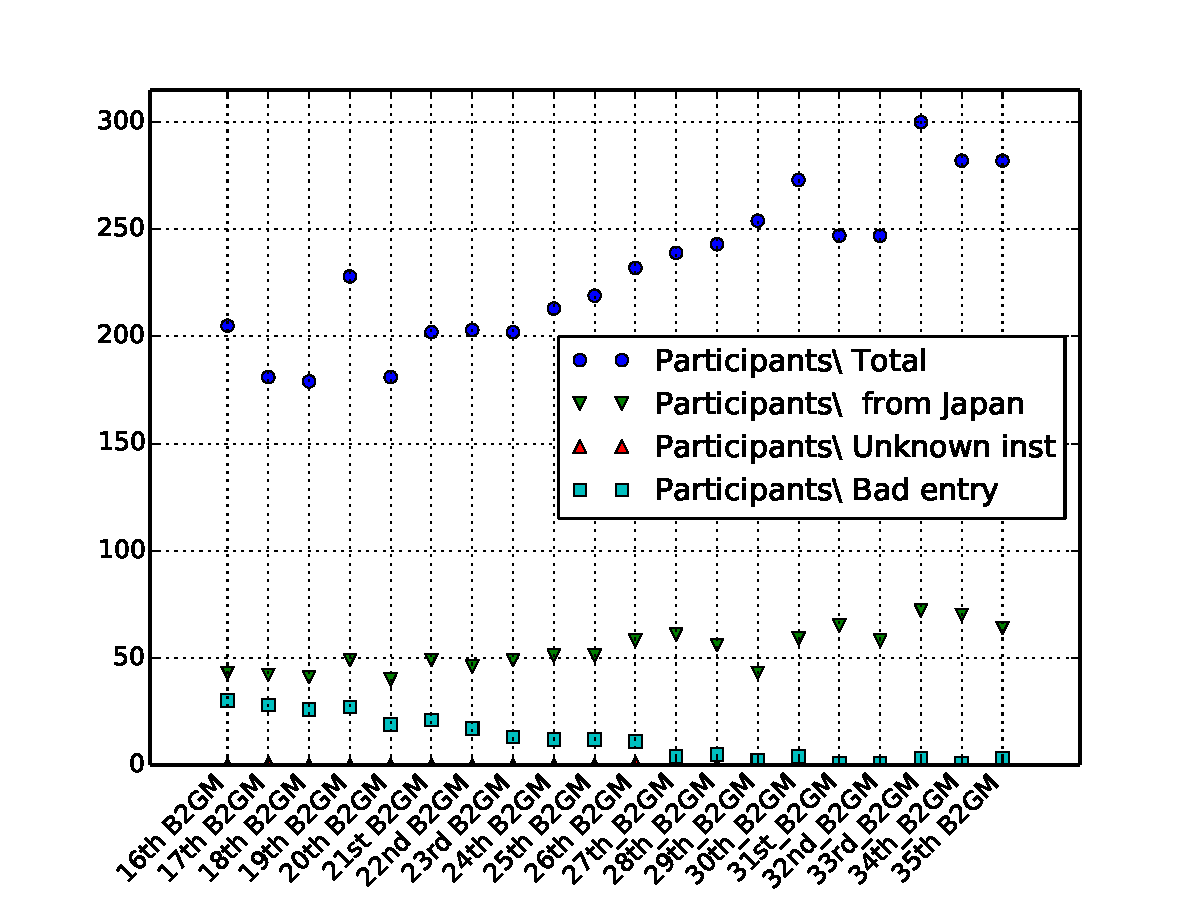
\includegraphics[width=\textwidth]{../FIGURES/B2GM_Participants.pdf}
\caption{Participants in B2GMs. }
\label{fig:B2GM_part}
\end{center}
\end{figure}

\begin{figure}[htbp]
\begin{center}
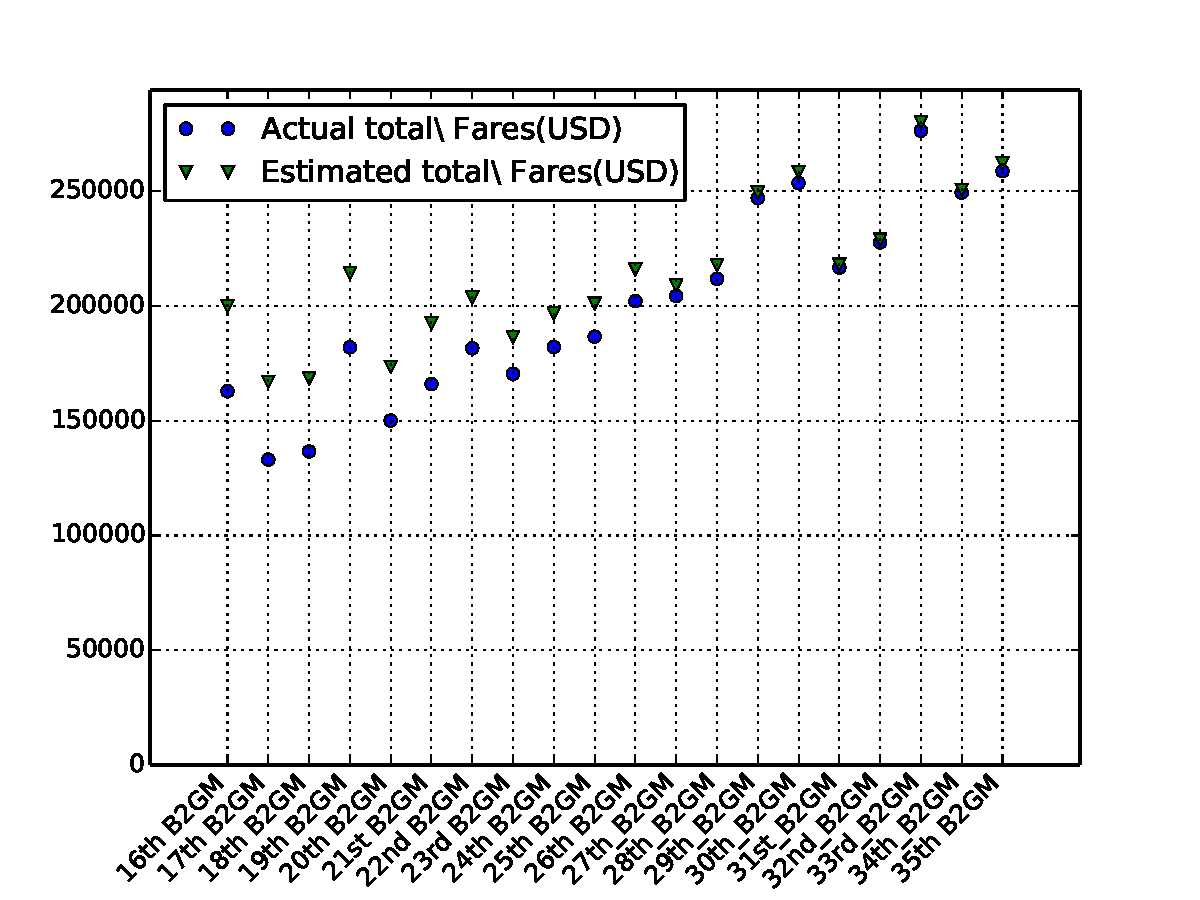
\includegraphics[width=\textwidth]{../FIGURES/B2GM_Fares.pdf}
\caption{Actual and estimated total airfare in USD for B2GMs. See text for details.}
\label{fig:B2GM_fares}
\end{center}
\end{figure}

 \begin{figure}[htbp]
\begin{center}
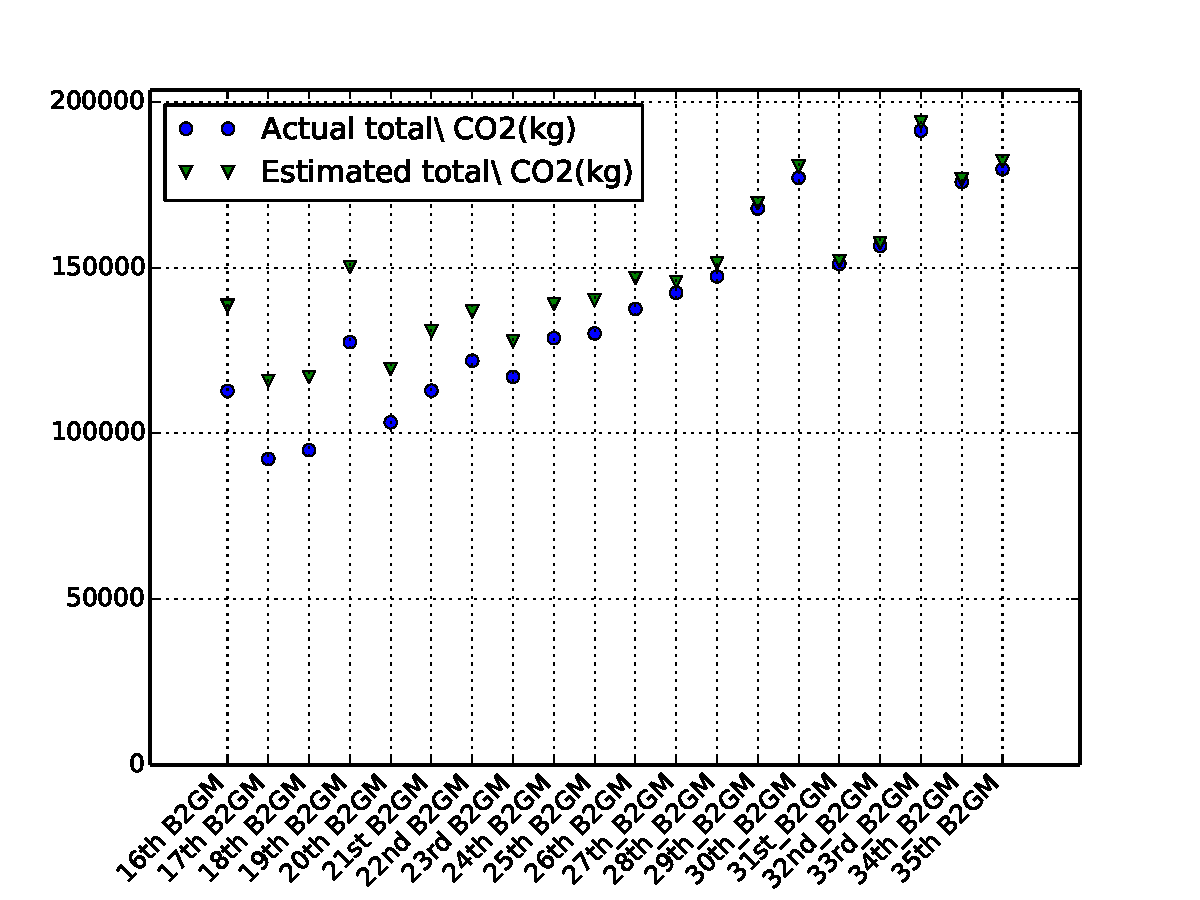
\includegraphics[width=\textwidth]{../FIGURES/B2GM_CO2.pdf}
\caption{Actual and estimated total \COtwo\ in kg for B2GMs. See text for details.}
\label{fig:B2GM_COtwo}
\end{center}
\end{figure}

 \begin{figure}[htbp]
\begin{center}
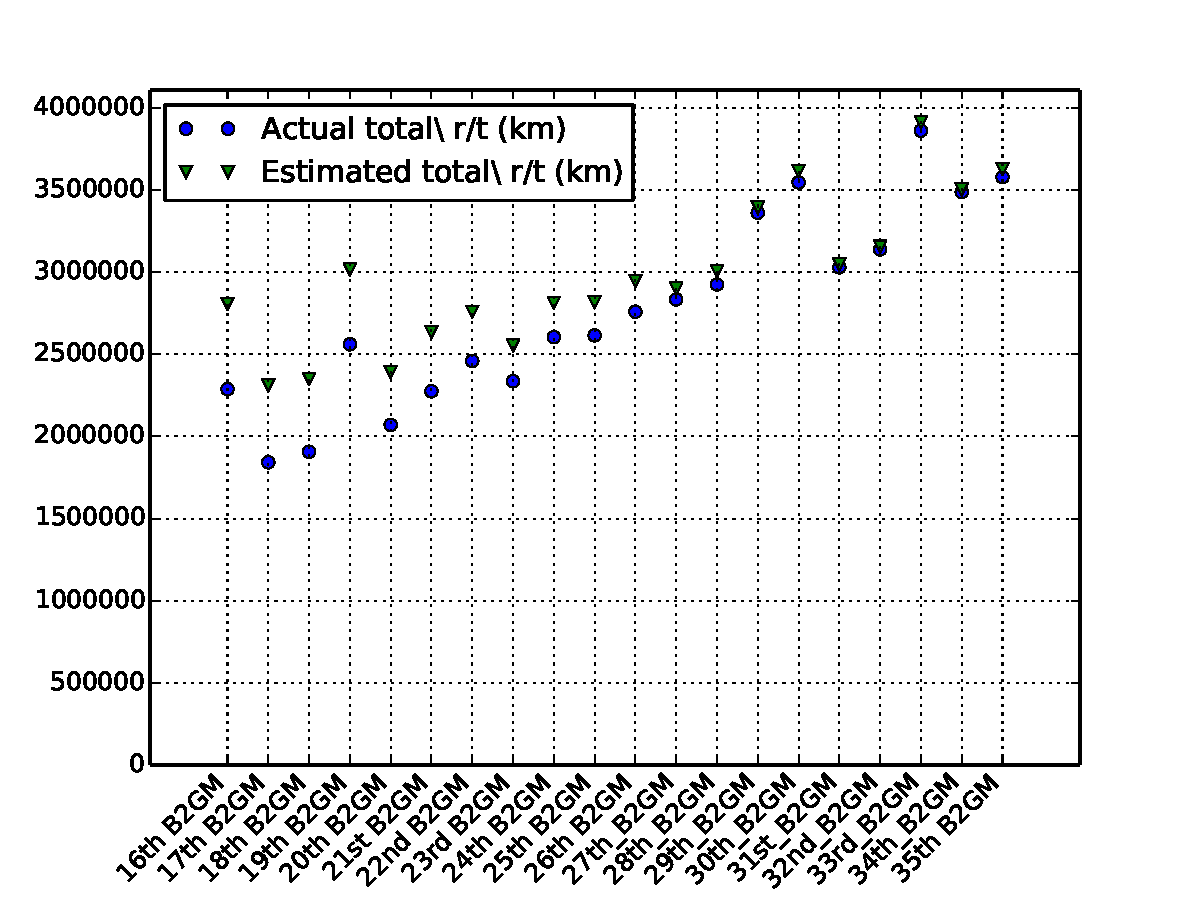
\includegraphics[width=\textwidth]{../FIGURES/B2GM_r-t.pdf}
\caption{Actual and estimated total round-trip air travel distance for B2GMs. See text for details.}
\label{fig:B2GM_r-t}
\end{center}
\end{figure}

\begin{figure}[htbp]
\begin{center}
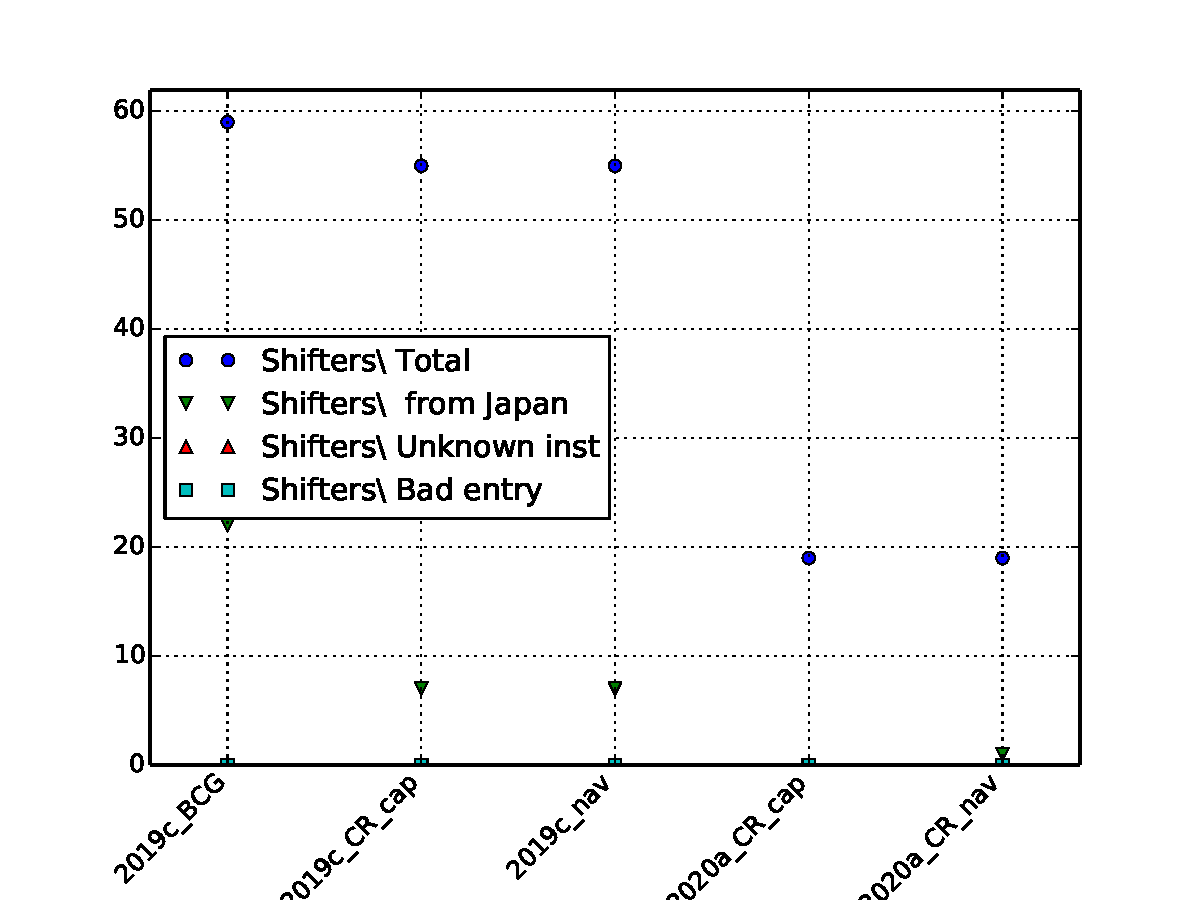
\includegraphics[width=\textwidth]{../FIGURES/Shifts_Shifters.pdf}
\caption{Actual and estimate total shifters for CR shifts. See text for details.}
\label{fig:Shifts_shifters}
\end{center}
\end{figure}

\begin{figure}[htbp]
\begin{center}
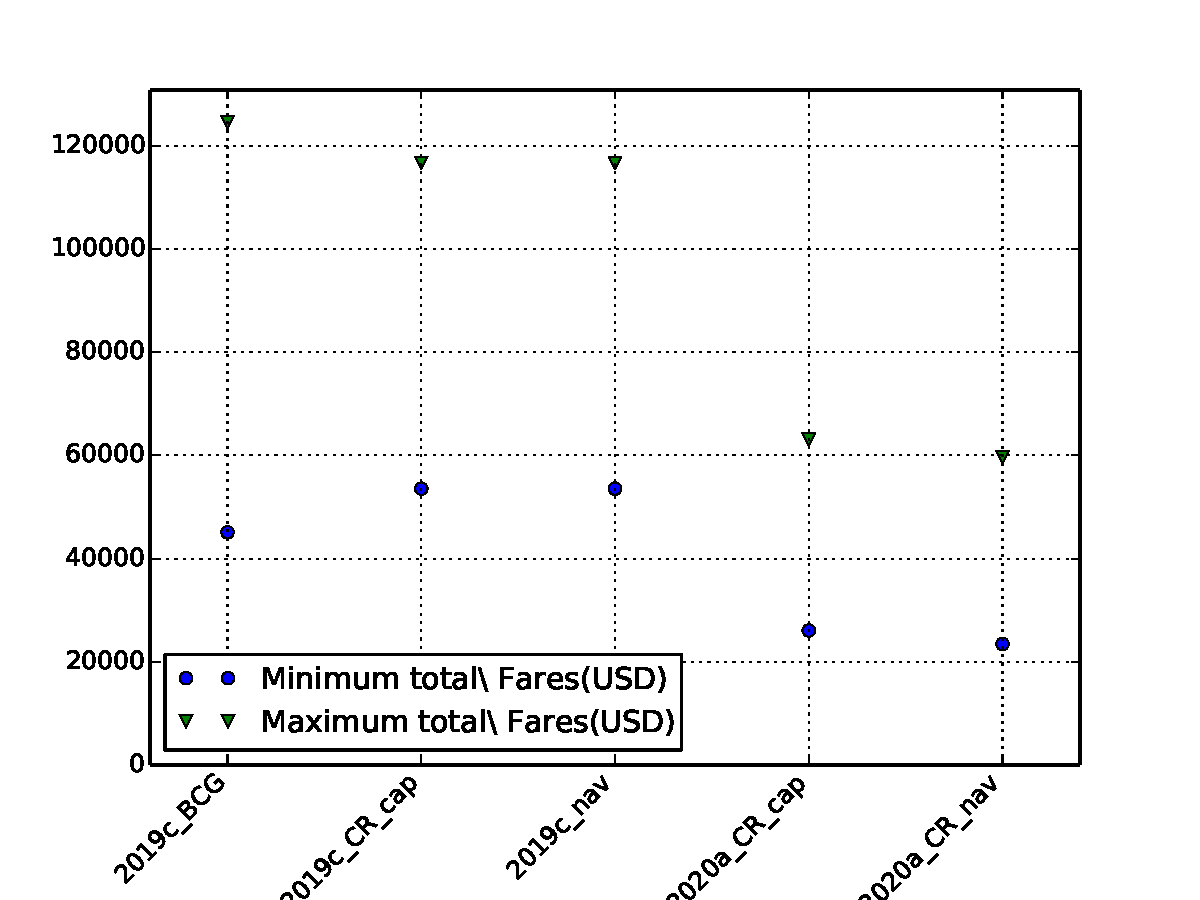
\includegraphics[width=\textwidth]{../FIGURES/Shifts_Fares.pdf}
\caption{Actual and estimated total airfare in USD for B2GMs. See text for details.}
\label{fig:Shifts_fares}
\end{center}
\end{figure}

\begin{figure}[htbp]
\begin{center}
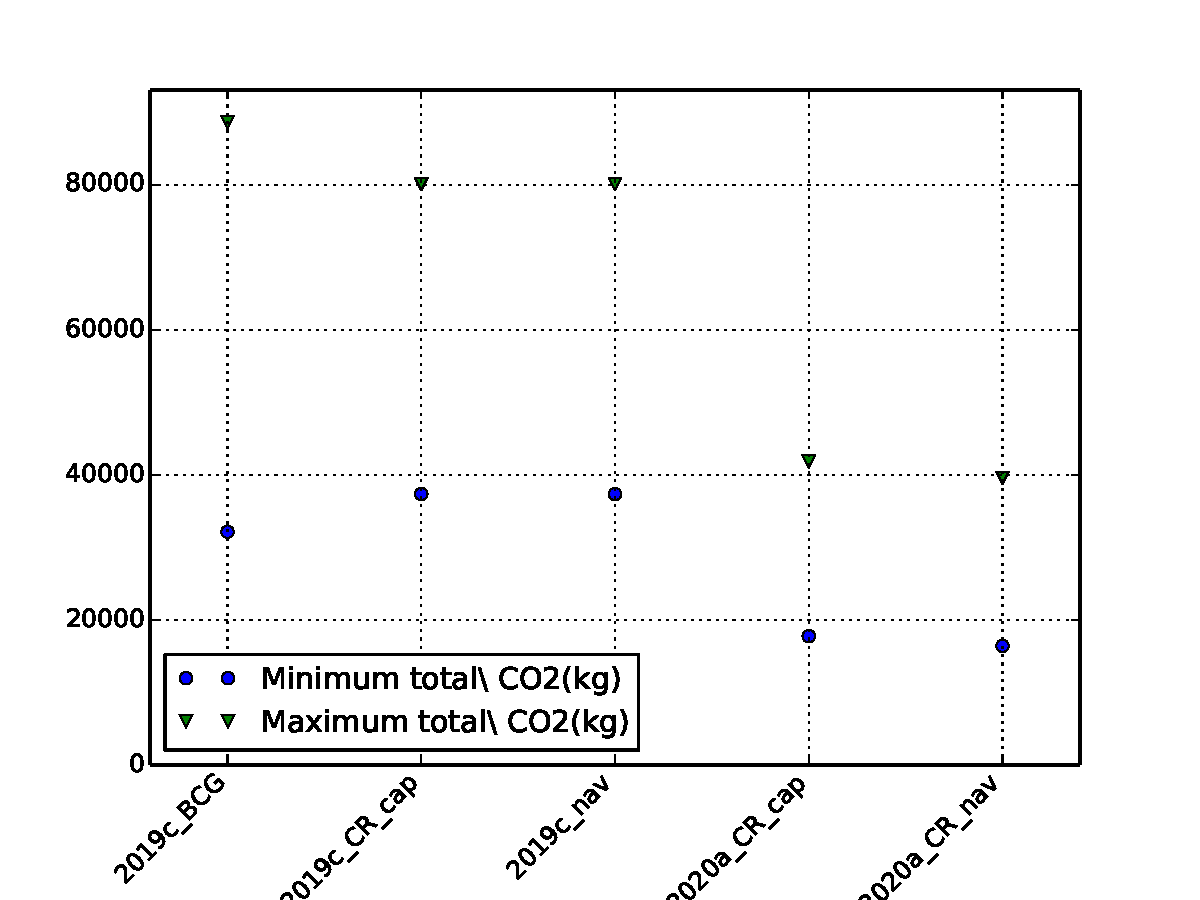
\includegraphics[width=\textwidth]{../FIGURES/Shifts_CO2.pdf}
\caption{Actual and estimated total \COtwo\ in kg for B2GMs. See text for details.}
\label{fig:Shifts_COtwo}
\end{center}
\end{figure}

\begin{figure}[htbp]
\begin{center}
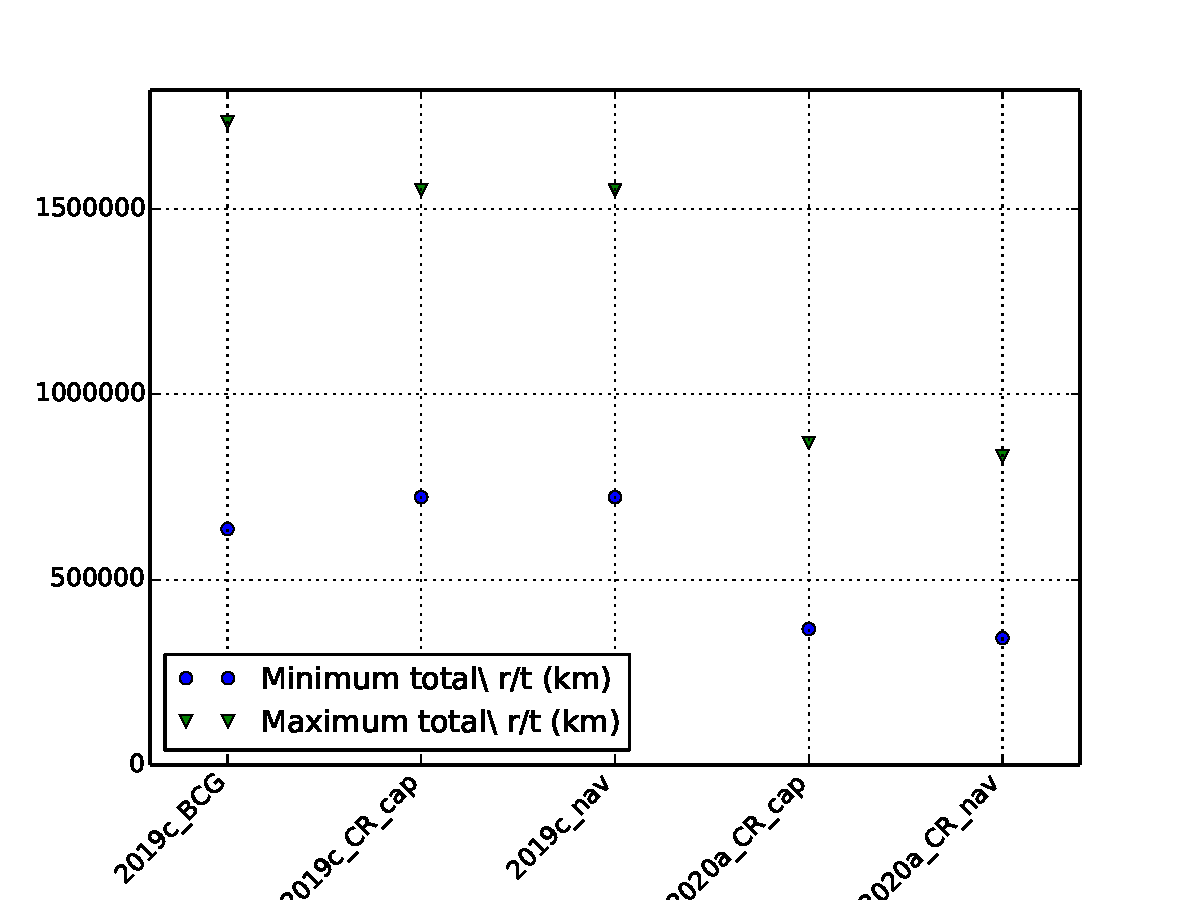
\includegraphics[width=\textwidth]{../FIGURES/Shifts_r-t.pdf}
\caption{Actual and estimated total round-trip air travel distance for B2GMs. See text for details.}
\label{fig:Shifts_r-t}
\end{center}
\end{figure}



\end{document}

